% This is "sig-alternate.tex" V2.0 May 2012
% This file should be compiled with V2.5 of "sig-alternate.cls" May 2012
%
% This example file demonstrates the use of the 'sig-alternate.cls'
% V2.5 LaTeX2e document class file. It is for those submitting
% articles to ACM Conference Proceedings WHO DO NOT WISH TO
% STRICTLY ADHERE TO THE SIGS (PUBS-BOARD-ENDORSED) STYLE.
% The 'sig-alternate.cls' file will produce a similar-looking,
% albeit, 'tighter' paper resulting in, invariably, fewer pages.
%
% ----------------------------------------------------------------------------------------------------------------
% This .tex file (and associated .cls V2.5) produces:
%       1) The Permission Statement
%       2) The Conference (location) Info information
%       3) The Copyright Line with ACM data
%       4) NO page numbers
%
% as against the acm_proc_article-sp.cls file which
% DOES NOT produce 1) thru' 3) above.
%
% Using 'sig-alternate.cls' you have control, however, from within
% the source .tex file, over both the CopyrightYear
% (defaulted to 200X) and the ACM Copyright Data
% (defaulted to X-XXXXX-XX-X/XX/XX).
% e.g.
% \CopyrightYear{2007} will cause 2007 to appear in the copyright line.
% \crdata{0-12345-67-8/90/12} will cause 0-12345-67-8/90/12 to appear in the copyright line.
%
% ---------------------------------------------------------------------------------------------------------------
% This .tex source is an example which *does* use
% the .bib file (from which the .bbl file % is produced).
% REMEMBER HOWEVER: After having produced the .bbl file,
% and prior to final submission, you *NEED* to 'insert'
% your .bbl file into your source .tex file so as to provide
% ONE 'self-contained' source file.
%
% ================= IF YOU HAVE QUESTIONS =======================
% Questions regarding the SIGS styles, SIGS policies and
% procedures, Conferences etc. should be sent to
% Adrienne Griscti (griscti@acm.org)
%
% Technical questions _only_ to
% Gerald Murray (murray@hq.acm.org)
% ===============================================================
%
% For tracking purposes - this is V2.0 - May 2012

\documentclass{llncs}

\usepackage{llncsdoc}
\usepackage{algorithmic}
\usepackage{algorithm}
\usepackage{graphicx}
%\DeclareCaptionType{copyrightbox}
%\usepackage{epsfig}
%\usepackage{epstopdf}
%\usepackage{url}
%\usepackage{multirow}
\usepackage{amsmath}
%\usepackage{amsthm}
%\usepackage{mathrsfs}
%\usepackage{enumerate}


\begin{document}


%
% --- Author Metadata here ---
\title{A Temporal Mining and Mixture Model for Residential Occupancy Prediction}

%\author{Huijuan Shao\inst{1} \and Yaowei Li\inst{2} \and
%Kamin WhiteHouse\inst{3} \and Naren Ramakrishnan\inst{1}}
%\authorrunning{Huijuan et al.} % abbreviated author list (for running head)
%\tocauthor{Huijuan Shao, Yaowei Li, Kamin WhiteHouse, and Naren Ramakrishnan}
%\institute{Virginia Tech, 900 North Glebe Rd., Arlington, VA, USA,\\
%\email{huijuans, naren@vt.edu},
%\and
%University of Virginia,
%501 Rice Hall, 
%Charlottesville, Virginia, USA \\
%\email{whitehouse@virginia.edu}}

\maketitle

%\numberofauthors{4} 
%\author{
% 1st. author
%\align author
%Huijuan Shao\titlenote{no note so far}\\
      % \affaddr{Virginia Tech}\\
       %\affaddr{900 North Glebe Rd.}\\
       %\affaddr{Arlington, VA, USA}\\
       %\email{huijuans@vt.edu}
% 2nd. author
%\alignauthor
%Yaowei Li\titlenote{The secretary disavows
%any knowledge of this author's actions.}\\
%       \affaddr{Game Source}\\
%       \affaddr{900 North Glebe Rd.}\\
 %      \affaddr{Arlington, VA, USA}\\
 %      \email{teadust@yeah.net}
% 3rd. author
%\alignauthor Kamin WhiteHouse\titlenote{The secretary disavows
%any knowledge of this author's actions.}\\
%       \affaddr{University of Virginia}\\
  %     \affaddr{501 Rice Hall }\\
     %  \affaddr{Charlottesville, Virginia, USA}\\
       %\email{whitehouse@virginia.edu}
%\and  % use '\and' if you need 'another row' of author names
% 4th. author
%\alignauthor Naren Ramakrishnan\titlenote{The secretary disavows
%any knowledge of this author's actions.}\\
 %      \affaddr{Virginia Tech}\\
   %    \affaddr{900 North Glebe Rd.}\\
     %  \affaddr{Arlington, VA, USA}\\
       %\email{naren@cs.vt.edu}
%}


%\maketitle
%\section{abstract}
Conserving energy and optimizing its use has been a long standing challenge. 
Apart from the monetary benefits associated with tackling these problems, saving energy has significant positive environmental impact. 
For instance, can the HVAC of residential buildings be adjusted automatically based on occupancy? 
In this work, we mine the people's energy activity profile to predict the occupancy of residential buildings. We propose a novel hybrid method, which uses episode mining for frequent events detection and associate them with Hidden Markov Model (HMM) to form a mixture of Episode Generating HMM (EGH) for target event prediction, 
combined with the standard kNN approaches and demonstrate how this hybrid approach always yields the best results.
%\section{abstract}

\chapter{Introduction}
\markright{Huijuan Shao \hfill Chapter 1. Introduction \hfill}

\emph{Analytics} has transformed the perception of the world we live in. Big Data is the lingua franca of the twenty first century and data science has become an essential lens through which decision making is seen. The massive amounts of data collected via several active and passive instrumentations positions us truly in \emph{age of information}. Data via Web 2.0, social media, internet of things, traffic flow, gene sequencing, etc. in conjunction with advancement of data mining & machine learning to glean actionable insights has influenced the world in designing policy, pricing products, launching political campaigns, and many other applications. The power of \emph{data analytics}, thus, is in its diversity. 

One such application is in \emph{urban computing}, primarily from the perspective of data science. It has been projected that by the year 2030, cities will grow by 590,000 square miles and add an additional 1.47 billion people, so that 6 out of every 10 people will live in a city. Key issues concerning urban populations, such as public health, sustainable use of limited energy resources, emergency preparedness, and societal stability will rise to the forefront. Epidemiological analysis of public health data to analyze infection spread, traffic flow analysis via public transport and taxi cab data, election forecasting and e-governance, and the like are just few of the many examples of how dissecting the data can provide awareness and knowledge about the society we live in. A data scientist role has become critical in being able to learn, process, analyze, and deliver actionable insights that can help realize the promises of this \emph{unprecedented urbanization}. 

Towards that end, one of the critical components which has long been a topic of research interest but has found resurgence in this era of urbanization is tackling problems of energy consumption. Sustainable energy supply to cities is more critical now than ever before. Moreover, the relevance of the problem is two-fold. The immediate impact of urbanization has presented us with logistical problems. How do we meet the needs of the rapidly growing cities? Can we design \emph{smart buildings} and \emph{smart neighborhoods} that optimizes energy consumption? Answering these questions is critical to the economy of the country and the economy of the society at large. The larger impact is one that energy industry has on the environment. While renewable energy sources are being investigated, fossil fuels remain the prime source of energy supply. Climate-change is a huge problem that will have an impact on humanity as we know it. It is a problem that needs a several pronged attack to find a solution and finding solutions to problems in energy consumption, reducing the carbon footprint, would be a big step forward.

One of the essential resources in today's world is power and electricity. Needless to say, electricity usage permeates all aspects of modern society.
Its most conspicuous
uses include urban contexts such as
lighting, air conditioning, refrigeration, heating, and, powering
appliances and gadgets but its penetration is pervasive across rural
and industrial sectors.
In 2014, the residential and commercial sector
comprised nearly 40\% of all the electricity generated in the U.S. \cite{book2014us}.
Furthermore, our dependence on electricity will continue to grow
as emphasis shifts away from fossil fuel based vehicles to electric
vehicles.

 

While people generally agree on the importance of conservation and
usage curtailment, they are often at difficulties to quantify 
{\em where, when} and {\em how much} electricity is consumed.
Typically, residences and businesses receive
monthly electricity bills indicating aggregate usage, with no information on
the breakdown of consumption by appliances/devices, time of day, or day of
week (this is an area in great flux, however). Research has 
shown that simply making such feedback available to users
can reduce consumption by up to 50\%, although typical saving 
are in the 9\% to 20\% range \cite{book2014us}.%\cite{energydatabook2011}.

One obvious approach to determining the breakdown of consumption is to install
power meters in every circuit (and sub-circuit)
to capture consumption of individual devices in homes and
offices. Such installation is costly and intrusive, making 
this option unviable in practice. 
An alternate
solution, called energy disaggregation or non-intrusive load monitoring
(NILM),
first proposed by Hart~\cite{hart1992}, is to use analytics to 
{\em infer} the breakdown of consumption from an aggregate 
power measurement of a
site. This drastically reduces the number of meters required per 
home/installation, typically to just one. Furthermore, depending on the analytics desired, it is possible to
use the measurements already being recorded by a utility meter for
disaggregation, especially in cases where utility companies have deployed
smart meters.
Energy disaggregation is hence today a booming area offering both
challenging problems for data analytics and having practical relevance in a
number of areas including sensor networks and building analytics.

Another approach to save energy in homes is to 
efficiently use electricity devices.  
In residential buildings, 
the biggest consumer of electricity is usually the HVAC 
(heating, ventilation, and cooling) system, which generally accounts for ~54\% 
of the buildings electricity consumption~\cite{book2014us}. 
How to automatically start up and shut down the HVAC unit 
is thus a key problem. 
One solution is to predict the occupancy at home 
is to begin by analyzing the activities of daily life 
inside the building. 
Based on the occupancy information, 
an automatic control system can be installed
to operate the HVAC. 

In this work we make efforts to resolve some of the problems arising in smart building research with 
temporal mining approaches.
\begin{enumerate}
	\item We present a survey on energy disaggregation from the perspective of data mining features and supervised, semi-supervised and unsupervised algorithms. 
	\item The temporal mining approach motif mining works effectively for energy disaggregation. 
	\item We utilize multivariate piecewise motif mining algorithm for both energy disaggregation and water disaggregation. 
	\item The episode-based model Episode Generating HMM (EGH) and a mixture of EGHs performs well for event prediction in occupancy prediction. 
	%\item It can be used for supervised learning disaggregation and semi-supervised learning approach, even for un-supervised learning approach. 
\end{enumerate}
\section{State of the art}
We open the thesis by defining energy disaggregation formally. Briefly, the goal of energy disaggregation is to effectively break down appliance level power consumption. We conduct a complete survey of several mechanisms and techniques that employ data mining and machine learning to tackle energy disaggregation. While surveys have been conducted in the past, most of them are presented from an electrical engineering perspective. We survey works that use supervised and unsupervised learning. We compare and contrast a range of algorithms that have been used for energy disaggregation. Our self-contained survey introduces the necessary electrical engineering concepts that are required for data scientists to conduct research in the space, describe necessary tools and datasets to develop and test algorithms. We describe how experimental testbeds should be setup and how to record data from the necessary sensors and meters. Moreover, we also present some promising directions of research in the space from a data mining perspective. Essentially, we provide a \emph{one-stop-shop} starting point for data mining practitioners to understand the problem scope of energy disaggregation, expose themselves to the problems, and then conduct research in the space.

\section{Temporal Mining}
One of the important forms of data is based on time. Temporal data mining revolves around the techniques (algorithms) that enumerate structures, patterns, and signatures over temporal data (time series, for instance). In this thesis we focus on three temporal mining algorithms. 

\subsection{Motif Mining}
Motif mining was a temporal data mining technique that was initially proposed in the \textbf{put motif mining cites} and it was extensively studied in \textbf{please put second motif mining cites}. Basically the fundamental idea behind \emph{motif mining} is that it symbolically encodes the numerical time series data. After which, the symbols combine to form episodes in the data resulting in patterns that can be mined. Furthermore by combining domain specific information and pattern mining techniques, we extract frequent meaningful episodes from the symbolized time series.

Furthermore when there are multiple time series that describe the data, we employ \emph{multi-variate motif mining} to find meaningful patterns. The algorithms for multi-variate temporal motif mining are similar to the univariate case, except that the symbolic encoding is represented as a vector. Therefore each time point in the data is represented as a vector of symbols, with each symbol corresponding to one of the several time series that represents the data. Now, the combination of these vector symbols forms episodes that can be mined from the multi-variate time series data. Again by combining domain specific knowledge, we extract meaningful episodes from the data.



\subsection{Episode Generating Hidden Markov Model (EGH)} A hidden markov model is an ubiquitous construct to model time series data. It is a tool for representing probability distributions over a sequence of data. The hidden Markov model gets its name from two important properties. The observation (data point) was generated by some process whose state is \emph{hidden} from the observer. Second, the state of this hidden process satisfies the \emph{Markov} property that the current state is independent of all prior states. The \emph{Episode Generating HMM}, researched in \textbf{put cites of EGH, please} connects the episodes with an HMM model and it has a parameter to evaluate whether an episode is frequent or not. A mixture of EGH describes a situation that several frequent episodes are embedded into a time series. It can be used to predict whether a target symbol will be the next symbol in a time series.



\section{Applications of Motif Mining and EGH}
In our work we apply motif mining techniques, both univariate and multivariate cases, to energy disaggregation. By correlating episodic information with the switching on and off of appliances from time-series represented energy data we are able to successfully determine the one-one mapping between a certain appliance and it's usage patterns and time. Our results are presented in Chapter 4.

The formulation of the EGH model lends itself to predicting occupancy in a residence or any building. We develop an EGH model based for occupancy prediction that can assist in automated turning on or off of the HVAC system, which can single-handedly reduce a good portion of the energy consumption footprint. We demonstrate that our algorithm can effectively forecast occupancy.  We present our analysis in Chapter 5.

The rest of the thesis is organized as follows. Chapter 3 presents a survey on energy disaggregation. Chapter 4 describes our solution to energy disaggregation and Chapter 5 discusses our solution to the occupancy prediction problem. We conclude the thesis in Chapter 6 with some discussion and future directions of research.  

%A related problem pertains to
%non-invasive indoor activities tracking.
%The goal here is to predict the locations of people inside a building
%without the use of invasive cameras.

%\section{Timeline}
%The first proposed
%research problem
%on energy disaggregation has been completed although 
%the work will be extended to time-based motif mining and 
%a new probabilistic models.
%The second task of activity of daily life patterns is underway. 
%The third subject on non-invasive indoor activities tracking 
%will start in this Oct.. 
%A timeline of activities is shown in Figure~\ref{fig_PhDtimeline}. 

%\begin{figure}[!hbtp]
%\centering
%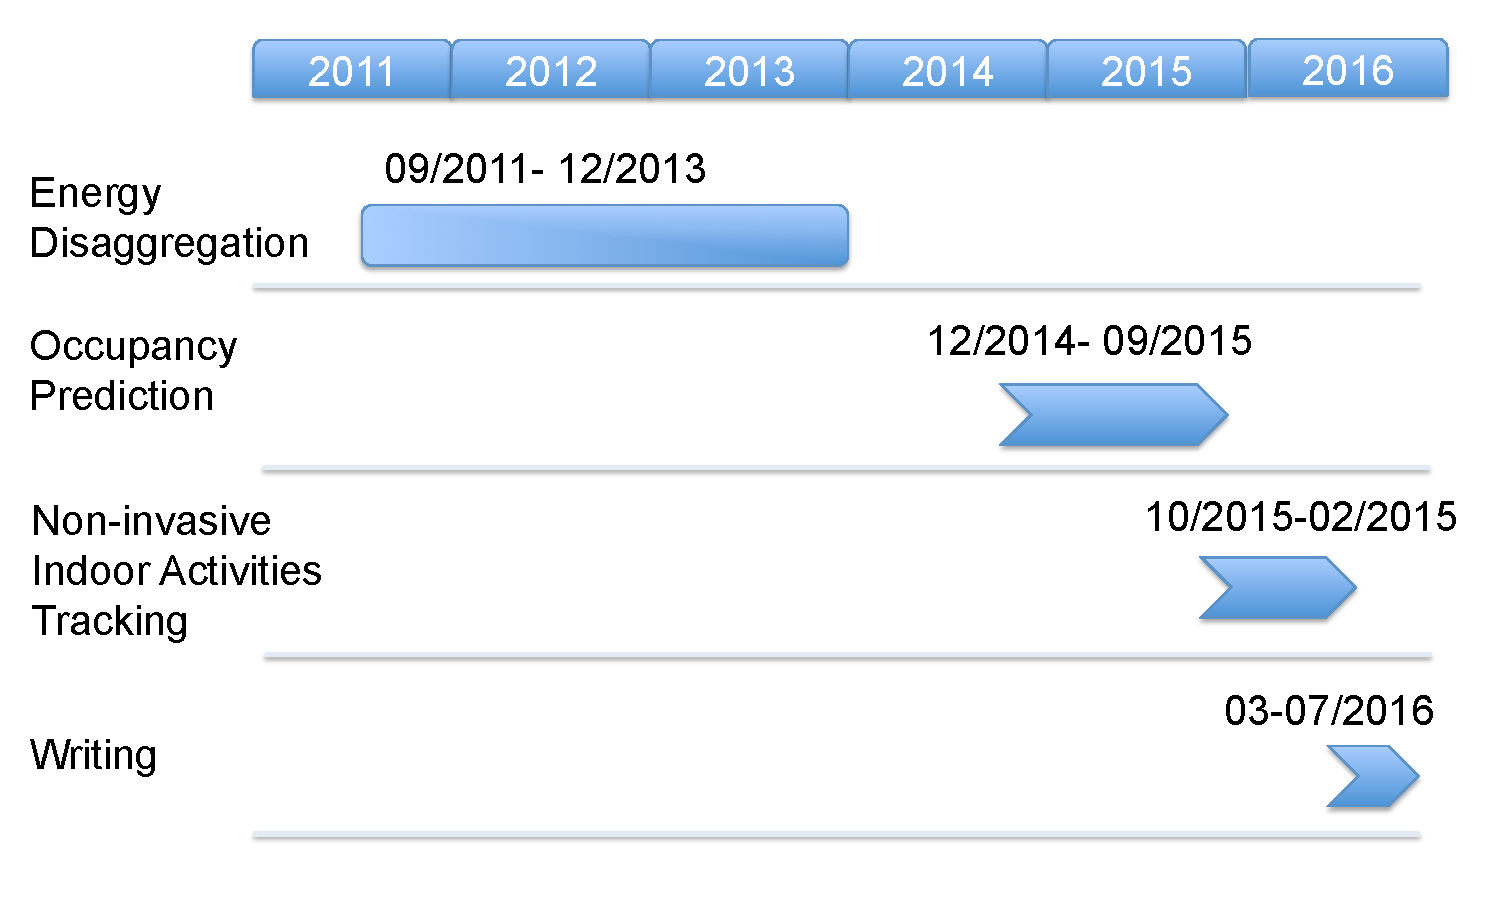
\includegraphics[width=0.8\textwidth]{fig/PhDTimeline.pdf}
%\caption{Timeline.\label{fig_PhDtimeline}}
%x\end{figure}

\section{Problem Formulation}
Before formalizing the problem statement, 
we introduce several concepts and notations first. 

\textit{Episode} An episode is a pattern which can be explained meaningfully. For instance, we represent 'S' as sleep, 
'K' as kitchen, and 'Z' as going out. 
If an episode $S \rightarrow K \rightarrow Z$ is found, 
the story is described as a person getting up, 
going to the kitchen for breakfast, and then leaving the house. 
An episode $\alpha$ is composed 
of a series of ordered events
$\alpha=\langle E_1,..,E_t,...E_n \rangle$, 
where $E_t$ denotes that $E$ occurs at time $t$.  
These events may be the point event or dwelling event. 
The dwelling event
has a start time $E.start$ and end time $E.end$. 
In this chapter  $E$ denotes a dwelling event and 
represents which room a person stays 
inside the building i.e is \emph{occupied}. 
For example we if $Z$ is used to show a room to be unoccupied. 
$Z.start$ means when the person goes out of home and 
$Z.end$ means when the person comes back. 

\textit{EGH} Episode generative HMM model is a 
type of HMM model which connects each episode $\alpha$ 
with a special HMM model $\Lambda_\alpha$. 
The uniqueness of the EGH is that 
the transition matrix and 
emission matrix is only decided by a noise parameter $\eta$. 
The value of $\eta$ is computed based on the frequency of the 
corresponding episode $\alpha$. 

We formulate the occupancy prediction problem as one of 
episode mining and event type time prediction problem. 

\textit{Problem Statement} Given a sequence of the room occupation 
events stream \textit{s} with finite events symbols $\varepsilon$, 
and the target un-occupancy event \textit{Z}, can we
find the frequent patterns $\{\alpha_1,...\alpha_n\}$ 
and can the corresponding episode generative HMM 
$\{\Lambda_{\alpha_1}, ..., \Lambda_{\alpha_n}\}$, 
predict when 
the person leaves $Z.{start}$, 
and when the person comes back $Z.{end}$.?

Next, 
we first discuss the time-gap constraint episode mining 
model and the mixture model, 
and how to predict the target event in section 4. 
Then, 
in section 5 we will show 
the experimental results. 

\iffalse
The training phase is to mine the frequent episodes and connect it with HMM model
as described in \cite{laxman2008stream}. We modify the constraints during episode mining
and keeps the connections between the frequent episodes and HMM the same. 
The training algorithm describes in Algorithm \ref{alg1}.
\fi

%% algorithm 01
\renewcommand{\algorithmicrequire}{\textbf{Input:}}
\renewcommand{\algorithmicensure}{\textbf{Output:}}

\begin{algorithm}
\caption{Trainng Algorithm}
\label{alg1}
\begin{algorithmic} [1]
\REQUIRE training events stream, $S_t=<\hat{E_1}, ..., \hat{E_n}>$; 
target event type Z; size of symbols $\varepsilon$ M; 
window size  \textit{W} preceding the target event Z
\ENSURE Generative model, $\Lambda_Z$ 

\COMMENT{re-organize data}\\
\STATE split data into each day
\STATE rename the symbol based on 15-minutes chuck
\STATE Initialize the partial stream $D_Z= \phi$ before $Z$

\FOR{the data of each day}
\IF{$\exists$ t that $\hat{E_t}=Z$}
\STATE add $S_t=<\hat{E_{t-W}}, ..., \hat{E_{t-1}}>$ to $D_Z$
\ENDIF
\ENDFOR

\COMMENT{build mixture episode generative HMM model}
\FOR{$1<w<W$}
\STATE mine the frequent episodes $\{\alpha_1, ..., \alpha_J\}$ 
\ENDFOR

\STATE connect each episode $\alpha_j $ with a HMM model EGH $\Lambda_{\alpha_j}$ 

\STATE generate episode generative HMM (EGH) mixture model $F(\Lambda)= \sum_1^J \theta_j\Lambda_{\alpha_j}$, where $1 \leq j \leq J$  
with EM algorithm

\STATE Output $\Lambda_Z=\{  (\Lambda_{\alpha_j}, \theta_j ) , j=1,...,J \}$

\end{algorithmic}
\end{algorithm}
\iffalse
From line 1-2, the symbols are reorganized according to the 15-minutes chuck of each day. 
If there are more than one symbols in a 15-minutes chuck, 
the symbol with longest duration event will be chosen. 
This step is to emphasize there is only one place a person stays in the room. 
From line 4-7, the W length sequence before the target symbol Z firstly appears is chosen 
for each day. 
From line 9-11, the frequent episodes are mined. 
From line 12-14, for each episode, a HMM model named EGH is generated and connected. Then a mixture model 
with all these EGHs are calculated with EM algorithm. 

The event time prediction algorithm Algorithm \ref{alg2} is composed of two stages. 
In the first stage from line 1-15,
we could predict whether the next event $E_{t+q}$ is the target event Z or not. 
For each $t$ is greater than W, intercept the sequence of length $W$ 
$X=<E_{t-W}, ..., E_t>$ in line 2. 
If Z is inside the X, then calculate the possible largest Z index $t_{max}$ inside X. 
In lines 4-6 the mixture model is calculated whether the next time $t+1$ would be the target event or not.
In line 8, all the frequent episodes will be checked whether it is inside the sequence X after $t_{max}$
If there is any frequent episode inside X, 
then we could predict the next event $E_{t+1}=Z$. 
That is, if any of the frequent episode happens 
and the value is greater than the threshold, 
then the next event is Z. 

In the second stage, the exact leave and back time prediction of Z is described from line 16-25. 
If a person gets up before sleep, 
generally we don't know when he will leave or come back. 
In this case, the predicted time is based on the average value of the past leave and back time. 
If a person already gets up, 
we mine the episode patterns, 
and predict according to the mixture model. 
This will be detailedly explained in \ref{alg22}.
If a person already leaves, 
the back time prediction is also based on the historical past time with 
a constraint on the leaving time. 
For a person may come back home and stay home for sometimes then go out again, 
we could repeat the second stage until the end of day. 
\fi
%% algorithm 02
\renewcommand{\algorithmicrequire}{\textbf{Input:}}
\renewcommand{\algorithmicensure}{\textbf{Output:}}

\begin{algorithm}
\caption{Prediction Algorithm}
\label{alg2}
\begin{algorithmic} [1]
\REQUIRE Partial day's event stream, $s=<E_1, ..., E_t, ...>$; 
target event type Z; size of symbols $\varepsilon$ M; 
window size  \textit{W} preceding the target event Z;
generative model $\Lambda_Z=\{  (\Lambda_{\alpha_j}, \theta_j ) , j=1,...,J \}$;
threshold $\gamma$

\ENSURE Predict $Z_{leave}$ and $Z_{back}$ if $E_{t+1}=Z$ or $E_{t+1}\neq Z$ 

\FOR{$W \leq t \leq len(s)$}
% get the stream inside a window W
\STATE set $X=<E_{t-W}, ..., E_t>$
\STATE $t_Z=0$

\COMMENT{the probability of X given the mixture model } \\
\IF{$P[X|\Lambda_Z] =\sum_1^J \theta_j\Lambda_{\alpha_j} \geq \gamma$} 

\IF{ $Z \in X$ }
\STATE Set $t_Z$ to largest  t, where $E_{t_{max}}=Z$ and $ t-W \leq t_{max} \leq t$
\ENDIF

\IF{$\exists \alpha \in \{\alpha_1,..., \alpha_J\}$ in X after $t_{max}$}
\STATE Predict $E_{t+1}=Z$
\STATE Record time of each symbol in these frequent episodes \\
%\COMMENT{calculate $\Delta t$ in Algorithm \ref{alg22}}
\ELSE
\STATE Predict $E_{t+1} !=Z$
\ENDIF
\ENDIF %end of the gamma
\ENDFOR

\IF{$E_{t+1} =Z$}

\IF{$t_Z$ happens before a person gets up}
\STATE $S_{leave}= \frac{\sum_1^J Z_{leave}}{J}$ where $Z_{leave}= t_{Z_{first}} \in \alpha_j$
\STATE $S_{back}= \frac{\sum_1^J Z_{back}}{J}$ where $Z_{back}= t_{Z_{last}} \in \alpha_j$
\ELSIF{$t_Z$ happens before a person gets up}
\STATE $S_{leave}$ and $_{back}$ are predicted by mixture models
\ELSE
\STATE $S_{back}= \frac{\sum_1^K Z_{back}}{K}$ where $Z_{leave}= t_{Z_{last}} \in \alpha_j$ 
and $Z_{leave}$ has a noise $\epsilon$

\ENDIF

\ENDIF
\STATE Output $E_{t+1}$, $S_{leave}$, $S_{back}$

\end{algorithmic}
\end{algorithm}





\section{Constraint Episode Mining and Mixture EGH}
We use a two-pronged approach to tackle the problem of mining and predicting unoccupancy.
First, we use an episode mining algorithm to discover frequent events before a person leaves 
a room. Then we use a mixture HMM model, EGH, to predict whether the room is unoccupied
and when the person leaves and comes back. 
%Then the possible time of the prediction  event will be predicted by averaging the past time. 

\subsection{Time-gap Constraint Episode Mining}
Episode mining has been studied in previous research \cite{mannila1997discovery} 
and \cite{laxman2005discovering}. 
Assume there is an event stream $s=ACBDEDEAABBA$, 
and the target episode is $AB$. To mine for $AB$, we can can use non-overlap mining approach to find the target episode. 
Non-overlap mining can be used where any two instances of the target episode has no intersection. It is to be noted that, non-overlap episode mining may result in different instances. 
For instance in the above example, if we align it to the left,  the episode mining results are $\langle A_1, B_3 \rangle, \langle A_8,B_{10} \rangle$. If aligned to the right, the results become as $\langle A_1, B_3 \rangle, \langle A_9,B_{11} \rangle$. 
A variant of episode mining is event gap constraint episode mining as proposed in
\cite{patnaik2008inferring}. 

In this application, 
the events dwell at an event for a period of time. 
Therefore, we combine the above two 
episode mining algorithms and enforce more constraints.
The first change is to 
use the right alignment for the first element in the episode. 
In the example of $AB$, 
the mined second instances is $\langle A_9,B_{11} \rangle$. 
The second modification is to 
check the time constraints and 
apply gap duration constraints between 
two consecutive events inside an episode. 
Figure \ref{fig_durationgapconstraint} shows an example of time-gap constraint episode. 
\begin{figure}[h]
\centering
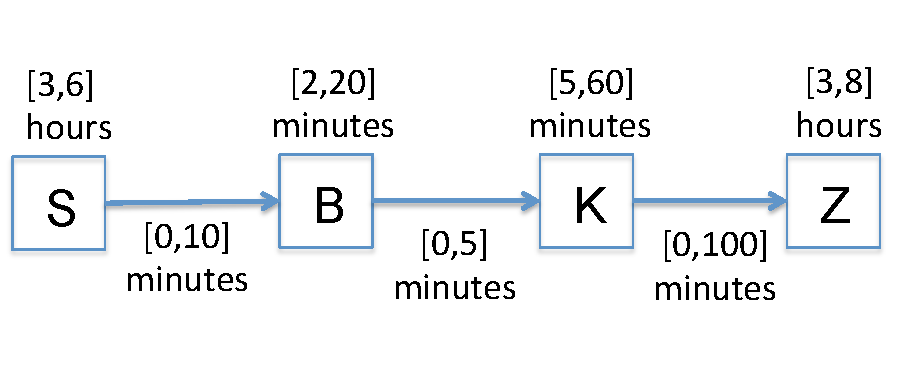
\includegraphics[width=0.7\textwidth]{adlfigs/durationgapconstraint.pdf}
\caption{Example of Duration-gap Constraint Episode.\label{fig_durationgapconstraint}}
\end{figure}

Assume we have the frequent episode $S\rightarrow B \rightarrow K\rightarrow Z$, 
we add the time constraints to each event $\{S,B,K,Z\}$. 
The dwelling duration of $S$ is 3 to 6 hours,   
of $B$ is 2 to 20 minutes, 
of $K$ is 5 to 60 minutes, 
and of $Z$ is 3-9 hours. 
Also, we set gap duration between any two consecutive events. 
The gap duration of $SB$ is calculated as $\Delta{SB} = B.start - A.end$. 
We set the maxim gap time between SB, BK, and KZ as 
10 minutes, 5 minutes and 100 minutes; 
the minimal gap time is 0. 
Figure \ref{fig_MingExample} is a time-gap constraint episode mining example. 
We have a stream composed of a sequence of dwelling events and the target 
episode is the same as in Figure \ref{fig_durationgapconstraint}.
The unit of the figures is in minutes.  
\begin{figure}[!hbtp]
\centering
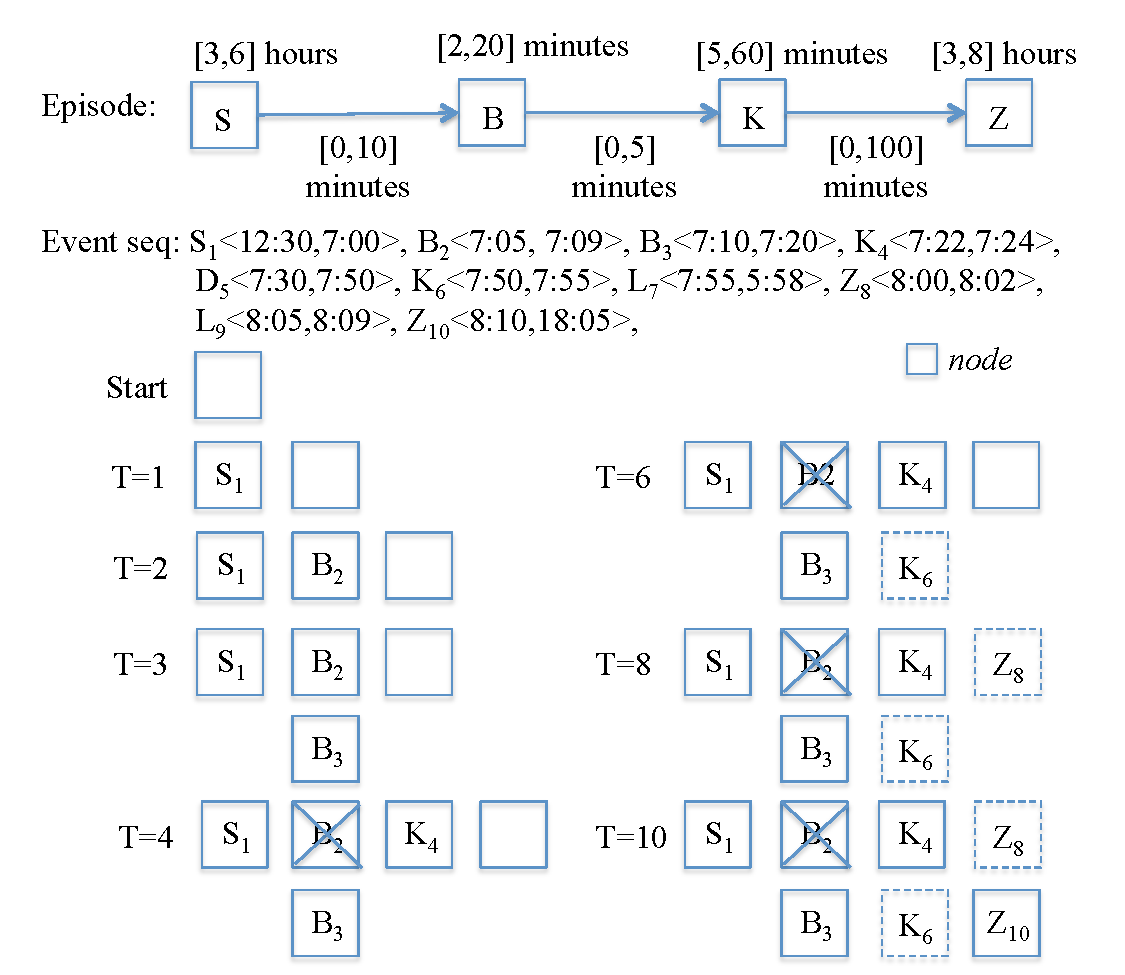
\includegraphics[width=1.0\textwidth]{adlfigs/MingExample.pdf}
\caption{Time-gap constraint episode mining example.\label{fig_MingExample}}
\end{figure}

Initially, a $waits$ structure related to this episode is created. 
Each $waits$ structure has the same length of episode structure $node$. 
A $node$ structure related to $S$ is created 
and it waits for the first 
element of the episode $S\langle 180, 360 \rangle $. 
When $T=1$, the duration of $S1$ is checked. 
Since it's in the range of $3-6$ hours, 
$S1$ passes and is put into the node structure $node$ related to $S$. 
Then a new $node$ structure is created to wait for $B\langle 2, 20 \rangle $. 
When $T=2$ and $T=3$, both of the $B2$ and $B3$ 
are qualified in terms of the time constraints and 
the gap constraints, 
e.g. the gap between $S$ and $B$ $\Delta SB$ should 
be between 0 to 10 minutes. 
Then $B2$ and $B3$ are input into the $node$ $B$ structure in the 
$waits$ structure. 
At the same time, 
a new $node$ structure is created for $K\langle 5, 60 \rangle $. 
When $T=4$, the gap between $\langle B3, K4 \rangle$ 
is satisfied with the distance condition between 
$B$ and $K$ 0-5 minutes. 
But the gap between $\langle B2, K4 \rangle$ 
is longer than the constraint gap. 
Therefore, $B2$ is canceled off. 
Now a new $node$ waits for the symbol $Z\langle 180, 540 \rangle$. 
When $T=6$, the gap from $B2$ and $K6$ is 
too far. Therefore, $K6$ is not added into the $node$ $K$ structure in $waits$.
When $T=8$, the time duration of $Z8$ is not qualified the condition between 3-9 hours. 
$Z8$ is not added. 
When $T=10$, the duration of $Z10$ meets the requirement 3-9 hours 
and its distance to $K4$ meet the requirement 
of $\Delta KZ \in [0,100]$ minutes. 
Thus $Z10$ is added into the $node$ $Z$ structure in $waits$.
Therefore, a complete episode mining is done. 

This complete gap-constraint episode mining on dwelling events 
is described in detail in Algorithm \ref{alg_episodeMiningConstraint}
%\ref{alg_episodeMiningConstraint_2e} 
in the appendix section.

%Non-overlap episode mining is defined as \textit{Definition}. 

\subsection{Episode Generating HMM}
Each frequent episode is connected with an HMM. 
According to EGH \cite{laxman2005discovering}, 
each episode generated HMM 
only has a noise parameter $\eta$.
The noise parameter $\eta$ of frequent episode $\alpha$ 
is calculated as $\eta=\frac{T-Nf_{\alpha}}{T}$ \cite{laxman2005discovering},  
where $T$ is the training data stream length, 
$\alpha$ is the frequent episode, 
$N$ is the length of frequent episode $\alpha$, 
$f_{\alpha}$ is the frequency over the time $T$.

Figure \ref{fig_egh} gives an example of the transition matrix in EGH. 
Assume we have a N-node frequent episode $S\rightarrow B\rightarrow Z$ and $N=3$ here.
We define 2N number of hidden states, 
N for episode states, and N for noise states. 
The noise states are $W\rightarrow X \rightarrow Y$. 
An episode state transfers to another episode state 
at the probability of $1-\eta$.
An episode state transfers to a noise state 
at a probability of $\eta$. 
A noise state transfers to another noise state 
at a probability of $1-\eta$. 
The emission matrix is calculated as following. 
Let M denote the totally number of symbols in the event stream. 
For any hidden states in the episode, it has a delta function emission. 
Whenever it is visited (right alignment of the first element in the episode, 
left alignment for the left elements in the episode), 
it will generate the same observation symbol. 
For any noise hidden states, it emits any of the symbols from the $M$ 
observation symbols with a uniform distribution at probability $\frac{1}{M}$. 

\begin{figure}[!hbtp]
\centering
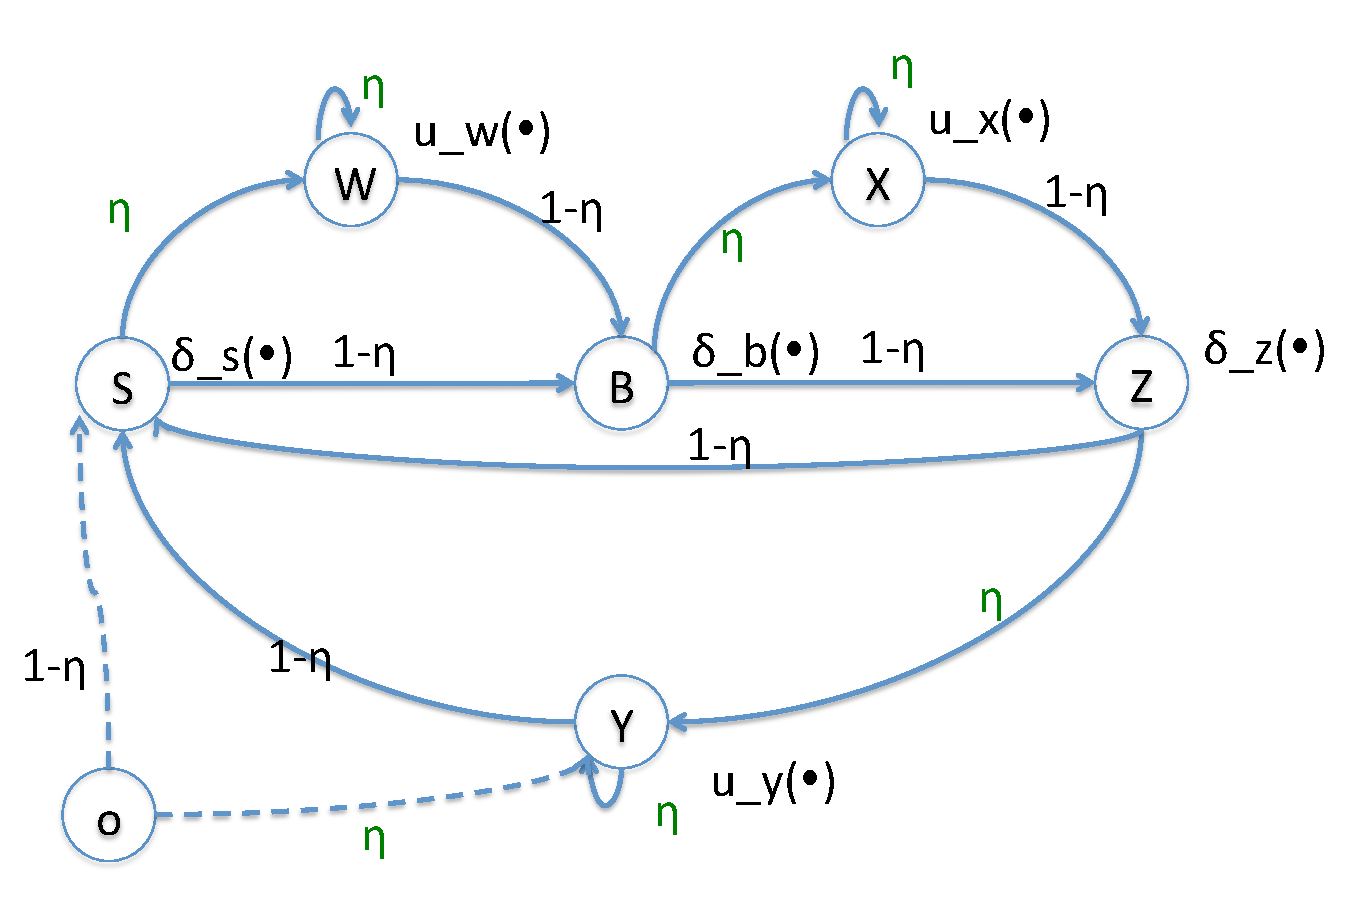
\includegraphics[width=0.7\textwidth]{adlfigs/egh.pdf}
\caption{States Transition of Episode Generating HMM (EGH).\label{fig_egh}}
\end{figure}


Theorem \ref{theorem1}~\cite{laxman2005discovering} is very important. 
It guarantees that the more frequent an episode inside the sequence, 
the probability of most likely sequence is larger. 
Its proof is explained in detail in \cite{laxman2005discovering}. 


\newtheorem{mydef}{THEOREM}
\begin{mydef}
\label{theorem1}~\cite{laxman2005discovering} 
Let $D_Z={X_1,..., X_K}$ is the given sequence data,  $\varepsilon$ is the symbol set, 
and the size of these symbols is $M$. 
Given two frequent N-node episodes $\alpha$ and $\beta$ with frequency $f_{\alpha}$ 
and $f_{\beta}$. Their corresponding EGH is $\Lambda_{\alpha}$ and $\Lambda_{\beta}$. 
The most likely state sequence for episode $\alpha$ and $\beta$ are
$q_{\alpha}^*$ and $q_{\beta}^*$. 
The noise parameters of these two EGH are 
$\eta_{\alpha}$ and $\eta_{\beta}$. 
Assume both of these noise parameters are less than $\frac{M}{M+1}$, 
we have 
(1) if $f_{\alpha} > f_{\beta}$, the $P(D_Z, q_{\alpha}^*| \Lambda) > P(D_Z, q_{\beta}^*| \Lambda)  $
(2) if $P(D_Z, q_{\alpha}^*| \Lambda) > P(D_Z, q_{\beta}^*| \Lambda)  $, $f_{\alpha} > f_{\beta}$
\end{mydef}

In this occupancy prediction application, 
we change the calculation of frequency. 
In our work, the frequency of episode 
is based on day. 
If an episode happens more than once, 
then we calculate it as only once. 

\subsection{Mixture EGH}
Mixture EGH has been discussed fully in previous work \cite{laxman2005discovering}.
The mixture EGH model has the advantage of 
giving different weight for each EGH model
for prediction. 
From the previous subsection, 
we obtain whether an episode occurs in a certain day. 
Let $D_Z=\{X_1,..., X_K\}$ denote the $K$ days data set. 
$F=\{\alpha_1, ... \alpha_J\}$ denote the frequent episodes in the dataset $D_Z$. 
EGH $\Lambda_{\alpha_j}$ 
corresponds to 
one of the frequent episode $\alpha_j$.
Let $\Lambda_Z$ denote the mixture model. 
The likelihood of $D_Z$ under the mixture model is written as Equation \ref{eq_mixture}.
\begin{eqnarray}
\label{eq_mixture}
Pr(\Lambda|Z) &=& \prod_{i=1}^K P[X_i|\Lambda_Z] \\
			&=& \prod_{i=1}^K ( \sum_{j=1}^J \theta_j P[X_i| \Lambda_{\alpha_j}])
\end{eqnarray}
where $\theta_j$ is the mixture coefficient of $\Lambda_{\alpha_j}$ and it subjects to 
$\sum_{j=0}^J \theta_j=1$ 

The parts inside Equation \ref{eq_mixture} are additive, 
the coefficients $\theta$ are computed by EM algorithm. 
The detailed description is algorithm %%%\ref{alg3} 
in the 
appendix section.
%% algorithm 03
\renewcommand{\algorithmicrequire}{\textbf{Input:}}
\renewcommand{\algorithmicensure}{\textbf{Output:}}

\begin{algorithm}
\caption{EM Algorithm for mixture EGH}
\label{alg3}
\begin{algorithmic} [1]
\REQUIRE day episode matrix, 
each element $e_{ij}$ records for each day whether an episode $j$ happens in day $i$;
frequent episodes $F=\{\alpha_1, ..., \alpha_J\}$;
symbol set $\varepsilon$;
threshold $\gamma$

\ENSURE the parameters for mixture EGH $\Lambda_Z=\{  (\Lambda_{\alpha_j}, \theta_j ) , j=1,...,J \}$


\STATE calculate the number of episodes J, and number of days K
\STATE calculate all $\eta$s' threshold value $mThreshold= \frac{M}{M+1}$

\COMMENT{initialize all the thetas to be $\frac{1}{J}$}
\COMMENT{calculate the total frequency for each episode over training time series}
\COMMENT{ calculate the $eta$ value}
\FOR{$0 \leq j \leq J$}
\STATE $\theta[j]= 1/J$
\STATE $episodeFreq[j] = \sum_i^K e_{ij}$
\ENDFOR

\STATE select those frequent episodes starting with 'S' and ending with 'Z' and separate these 
episodes by workday or holiday

\COMMENT {calculate $eta$ for each episode} 
\FOR{$0 \leq j \leq J$}
\STATE $\eta[j]= 1-episodeLen[j]*episodeLen/T$
\ENDFOR

\COMMENT{likelihood prediction of each episode $j$ in the $k$th day}

\FOR{$0 \leq i \leq K$}
\FOR{$0 \leq j \leq J$}
\STATE $likelihood_{ij} = \frac{1-\eta[j]}{\eta[j]/M} ^ {episodeLen[j]*e_{ij}}$
\ENDFOR
\ENDFOR

\COMMENT{calculate the obj value based on J, K, $likelihood_{ij}$ and $\theta$}
\WHILE{$newObj- obj > \gamma$}
\STATE $\theta_{new}=[]$
\FOR{$0 \le l \le J$}
\STATE $temp=0$
\FOR{$0 \le j \le K$}
%\COMMENT{calcuate the new likelihood with Bayes rules}
\STATE $temp = temp+ \frac{\theta_l*likelihood_{il}}{ \sum_0^J { \theta_j*likelihood_{ij}}}$

\ENDFOR
\STATE $\theta_{new}[l] = temp/K $
\ENDFOR

\STATE calculate the newObj
\IF{$newObj-obj > \gamma$}
\STATE $obj=newObj$
\STATE $\theta_{new} = \theta$
\ENDIF

\ENDWHILE

\STATE Output $\Lambda_Z=\{  (\Lambda_{\alpha_j}, \theta_j ) , j=1,...,J \}$

\end{algorithmic}
\end{algorithm}
During the initialization %line 1-10
part of the EM algorithm, 
the episode frequency over the times series T is calculated. 
Specific frequent episodes ended with target event 'Z' are selected. 
Optionally, 
we could add special constraints on episodes starting with 
certain event type 'S'. 
%calculated in lines 11-16. 
In the expectation step, 
one key part is the likelihood value of each episode $\alpha_j$ in time series $X_i$.
The likelihood value is computed as Equation \ref{eq_likelihood}.
Then Bayes rules is applied to compute the new coefficient $\theta_{new}$. 
\begin{equation}
\label{eq_likelihood}
Pr(X_i| \Lambda_{\alpha_j}) = (\frac{\eta_{\alpha_j}}{M})^{|X_i|} (\frac{1-\eta_{\alpha_j}}{\eta_{\alpha_j}/M})^{|\alpha_j|f_{\alpha_j}(X_i)}
\end{equation}
In the step of maximization, 
we can update the objective value based on Equation \ref{eq_mixture}. 
and until it converges, i.e., 
the difference of two consecutive objective values 
is smaller than a threshold.%$\gamma$.

\subsection{Predict When the Target Event Occurs}
Target event prediction has been studied in  \cite{laxman2008stream}. 
But it only predicts whether a target event will occur or not. 
It never considers when the target event will happen. 
The occupancy prediction problem involves three sub-problems: 
1) whether the target event un-occupancy $Z$ will appear; 
2) when the target event $Z$ starts; 
3) when the target event $Z$ ends. 

For stream prediction for target event, 
refer to algorithm in \cite{laxman2008stream}. 
This section emphasizes on the last two sub-problems, 
predicting when the person leaves  $Z_{leave}$ or comes back $Z_{back}$ 
after we already know target event $Z$ will surely happen. 
Note that $Z_{leave}$ corresponds to $Z.start$, when the $Z$ event starts. 
$Z_{leave}$ corresponds to $Z.end$, when the $Z$ event ends. 
This prediction algorithm is described in algorithm \ref{alg22}. 

After running episode mining and mixture EGH model, 
we have obtained all the frequent episodes $F=\langle \alpha_1,..., \alpha_J \rangle$, 
the corresponding EGH $\Lambda_{\alpha_j}, j=1...J$ with noise parameter $\eta_j$, 
and the mixture models $\Lambda_Z$ with coefficients $\theta_j$.
We use the coefficient of these mixture models for leave time and back time prediction. 
The algorithm \ref{alg22} 
uses partial day of test data $s$, 
all the frequent episodes  $epis$, 
the frequent episodes $F$ in partial day of $s$, 
the mixture model $\Lambda_Z$, 
to predict when the person leaves or comes back home. 
The partial day is cut by partial index $pIndex$. 
Each day is cut into three phases, before the person gets up; 
after the person gets up but before the person leaves home;
after the person comes back home. 

In the first two phases, before the person leaves, 
the PDF leave time and back time are calculated from line 2-4. 
Usually before a person gets up, there is only one frequent episode named 'SZ'. 
After the person gets up, he/she has a lot of activities at home, 
there are several frequent episodes mined before the person leaves home. 
In case there are several frequent episodes in lines 6-12, 
the leave time and back time of each episode is checked
whether they are in a range of PDF value in the past. 
If yes, the mean value of these episodes are recorded from line 14-17. 
If there are several frequent episodes with corresponding EGH, 
the leave time $Z_{leave}$ and back time $Z_{back}$ is the weighted 
mean leave time and back time of each episode in lines 18-21. 

In the third phase, after the person leaves home, 
we already know when the person leaves home $Z_{leave}$ 
but needs to predict when the person comes back $Z_{back}$. 
If the person has come back, that means $Z_{back}$ is not equal to $Z_{leave}$. 
We don't need to do anything. 
If the person has not come back, that means $Z_{back}$ equals to $Z_{leave}$. 
The back time is the past weighted back time from line 28-34. 

% algorithm 22, an extention of algorithm 2
\renewcommand{\algorithmicrequire}{\textbf{Input:}}
\renewcommand{\algorithmicensure}{\textbf{Output:}}

\begin{algorithm}
\caption{ Target Event Occurs Time Prediction Algorithm}
\label{alg22}
\begin{algorithmic} [1]
\REQUIRE 
partial day cut point $pIndex$, $s[1:pIndex]$ is known,  and $s[pIndex:96]$ for prediction;
partial day event stream $s=\langle E_1,..., E_{pIndex} \rangle$;
all the episodes $epis$, $\forall E \in \alpha$ and $\forall \alpha \in epis$, E has $E.{start}$ 
and $E.{end}$; 
frequent episodes $F=\langle \alpha_1,..., \alpha_J \rangle$ inside $s[1:pIndex]$;
EGH model $\Lambda_{\alpha_j}$ with noise parameter $\eta_j$ where $j=1...J$
EGH mixture model coefficients $\Theta=\langle \theta_1,...,\theta_J \rangle$;
the slot number noise parameter $\epsilon$  ; 
target event $Z$
\ENSURE Predict target event leaving time $Z_{leave}$ and back time $Z_{back}$
 
\IF{$Z  \notin s $}%\COMMENT{predict before the person leaves home}
\STATE choose episodes $\alpha.ev={'SZ'}$ 
\STATE $Z_{leave} = \frac{\sum_1^K Z.start}{|\alpha|} $
\STATE $Z_{back} = \frac{\sum_1^K  Z.end}{|\alpha|}  $
\IF{$len(F)>1$}%\COMMENT{if there are several episodes to predict 'Z'}
\FOR{$\alpha_j \langle e_1,..., e_j \rangle \in F$}
%\IF{$\alpha_j.ev='SZ'$} % 'SZ' has been calculated,no need to calculate again
%\STATE break
%\ENDIF
\IF{$pIndex \in ( \alpha_j. ev[-2].start - \epsilon, \alpha_j.ev[-2].start+ \epsilon )$}
\STATE $leaveMap[\alpha_j.ev]=\alpha_j.leave$
\ENDIF
\IF{$pIndex \in ( \alpha_j. ev[-2].end - \epsilon, \alpha_j.ev[-2].end+ \epsilon )$}
\STATE $backMap[\alpha_j.ev]=\alpha_j.back$
\ENDIF 
\ENDFOR
\IF{$len(leavingMap) !=0 $} % for the average
\STATE $leaveSlotMap[\alpha_j.ev] =\frac{\sum_1^K leavingMap.get(k)}{K}$
\STATE $backSlotMap[\alpha_j.ev] = \frac{\sum_1^K backMap.get(k)}{K}$
\ENDIF % this is for the len\\
\IF{$K=len(leaveSlotMap)>1$}%\COMMENT{There are other frequent episodes except 'SZ'}
\STATE $Z_{leave}= \frac { \sum_{k=1}^K leaveSlotMap.get(k) * \theta_k } {K}$
\STATE $Z_{back}= \frac { \sum_{k=1}^K backSlotMap.get(k) * \theta_k } {K}$
\ENDIF
\ENDIF %this is for len(F)>1 
\ENDIF %this is for if Z \notin S \\
\IF{$Z  \in s $}%\COMMENT{if the person has left home}
\STATE $Z_{leave}=s.firstindex[Z]$ % the position where $Z$ first appears
\STATE $Z_{back}=s.lastindex[Z]$ % the position when $Z$ lastly appears\\
%\STATE backSlotMap=\{\}
\IF{$Z_{leave}=Z_{back}$} %\COMMENT{The person hasn't come back}% the person hasn't come back
% get the average of those time
\FOR{$\alpha_j \langle e_1,..., e_j \rangle \in F$}
\IF{$Z_{leave} \in [\alpha_j.ev[-2].end - \epsilon, \alpha_j.ev[-2].end + \epsilon ]$}
\STATE $backSlotMap[\alpha_j.ev] = \alpha_j.leave$
\ENDIF
\ENDFOR
\STATE $Z_{back}= \frac { \sum_{k=1}^K backSlotMap.get(k) * \theta_k } {K}$
\ENDIF
\ENDIF
\STATE Output the slot number when the person leaves $Z_{leave}$ and comes back $Z_{back}$
\end{algorithmic}
\end{algorithm}
 






\section{Experiment Results}
We have conducted experiments on three datasets, where each dataset is obtained by monitoring 24-hour activities of two adults in a house through RFID.
The dataset comprises of events which are timestamped room occupancy data points. For instance, an event can correspond to person 1 being in the kitchen at 7:00 am. The summary of these three datasets is shown in table~\ref{tab_dataset}. 
\begin{table}[h]
\centering
\caption {Datasets summary.} \label{tab_dataset}
%\vspace{0.2cm}
\begin{tabular} {|l|l|c|}
\hline
Dataset  & Period & Number of people \\
\hline
study10 & 12 days & 2 \\
\hline
study11 & 10 days & 2 \\
\hline
study14 & 13 days & 2 \\
\hline
\end{tabular}
%\end{center}
%\end {table}
%\end{minipage}%
\end{table}
Study10 spans 12 days from 02/10/2014 to 02/21/2014 and Study11 spans 10 days from 01/29/2014 to 02/07/2014, and Study14 spans 13 days from 12/09/2013 to 12/21/2013.

We define \textit{unoccupancy} of a person as follows: 1) the person leaves the {\em outside-front} or {\em outside-back} for more than 30 minutes; 2) the person stays in the living room or dining room for more than 9 hours without any other activities; 3) the gap between any two events is more than 30 minutes. 
Since our research goal is to automate the turning on and off of the HVAC system at least 30 minutes before occupancy, the first and third constraints are in place. We are only interested in events where the {\em unocupancy} period is for an extended duration (> 30 minutes). The second constraints comes from our observation that if a person stays in one room for more than 9 hours without moving to other rooms, 
usually it means that the person goes out by leaving the RFID equipment at home. 
We delete events with duration less than 
2 minutes since these correspond to the individual walking back and forth across rooms and generally do not contribute to meaningful episodes. We conduct three types of experiments to compare three approaches, 
kNN, mixture EGH and Probability Density Function (PDF). 
For each dataset, we use $2/3$ data for training and the left $1/3$ for test. 
Following the approach in~\cite{scott2011preheat},
we organize one day's date into 96 15-minutes. 
For test data, we assume that we only know partial number of 15-minutes' chunks. Our target is to predict the occupancy in the rest of the day, or 30-minutes ahead. 

\subsection{Occupancy Prediction of Individuals}
%We apply three approaches, kNN, PDF based and mixture EGH time prediction model. 
%Similar to \cite{scott2011preheat},
%we organize one day's date into 96 15-minutes intervals with mixture EGH model. 
%Then we split the test date into three phases: 
%(1) before getting up, (2) after getting up and before going out, 
%(3) after going out and before coming back. 
%Thus our problem becomes to predict when the person going out 
%and when the person comes back. 
%Corresponding to these four phases, we adopt three different approaches. 
%For stage (1), the probability density function of going out and combing back event is calculated. 
%For stage (2), a duration-constraint episode mining and episode generative HMM is applied. 
%For stage (3), the probability density function of backing time based on 
%the time-constrains going out time is computed. 

%The results are shown in Figure~\ref{fig_study10} and Table~\ref{tab_individualResults}
%Figure~\ref{fig_study11}, and Figure~\ref{fig_study14}. 
%Each of these figures 

\begin{table*}[t]
%\vspace{0.2cm}
\hfill
\begin{minipage}[t]{1.0\linewidth}%

\caption{Precision Recall F-measure Comparison of Individual and Whole House Occupancy Prediction.}
\label{tab_individualResults}
\begin{center}
\makebox[\textwidth]{
\begin{tabular} {|l|l|l|l|l|l|l|l|l|}
\hline
\multirow{2}{*}{Dataset}&\multirow{2}{*}{Date}&\multirow{2}{*}{Person} & \multicolumn{3}{|c|}{EGH}&\multicolumn{3}{|c|}{kNN}  \\
\cline{4-9}
&&& Precision & Recall &F-measure &Precision & Recall & F-measure  \\
\hline
\multirow{3}{*}{study10}  & 02/17/2014 & person2& \textbf{1.00} & \textbf{1.00}&\textbf{1.00} & 0.99 & 0.98 & 0.98\\
\cline{2-9}
& 02/19/2014 & person1& 0.98 & 0.99 &0.98&  \textbf{0.99} &  \textbf{0.99} &  \textbf{0.99} \\
\cline{2-9}
& 02/20/2014 & person2&  \textbf{0.93} &  \textbf{0.92} &  \textbf{0.92} & 0.92 & 0.91 & 0.90 \\
\cline{2-9}
& 02/20/2014 & person1&  \textbf{0.95}& \textbf{0.94} & \textbf{0.94} & 0.94	& 0.93 & 0.93 \\
\cline{2-9}
& 02/20/2014 & \textbf{whole-house}&  \textbf{0.92}& \textbf{0.92} & \textbf{0.91} & 0.91	& 0.89 & 0.91 \\
\hline
\hline
\multirow{3}{*}{study11}  & 02/04/2014 & person2& 0.93 & 0.93 & 0.92  & \textbf{0.95} & \textbf{0.95} & \textbf{0.95}\\
\cline{2-9}
& 02/04/2014 & person1& 0.93 & 0.93 & 0.92  & \textbf{0.95} & \textbf{0.95} & \textbf{0.95} \\
\cline{2-9}
& 02/05/2014 & person2&  \textbf{0.85} &  \textbf{0.92} &  \textbf{0.86} & 0.87 & 0.87 & 0.84 \\
\cline{2-9}
& 02/05/2014 & person1&  \textbf{0.84} &  \textbf{0.90} &  \textbf{0.84} & 0.79 & 0.90 & 0.80 \\
\cline{2-9}
& 02/04/2014 & \textbf{whole-house}&  \textbf{0.918}& \textbf{0.924} & \textbf{0.913} & 0.916	& 0.921 & 0.911 \\
\cline{2-9}
& 02/05/2014 & \textbf{whole-house}&  \textbf{0.90}& \textbf{0.84} & \textbf{0.84} & 0.88	& 0.81 & 0.81 \\
\hline
\end{tabular}
}
\end{center}
\end{minipage}%
%\hfill%
\end{table*}
The individual occupancy prediction results on datasets Study10 and Study11 are summarized in table~\ref{tab_individualResults}. 
In Study10 as to the occupancy prediction for person2 on 02/17/2014, the mixture EGH performs better than kNN. 
Also, mixture EGH outperforms kNN for both persons on 02/20/2014. 
However, for person1 on 02/19/2014, kNN works a little bit better. 
When checking the original date on this test date, 
we find that the activities on this date is very similar to the historical activities in the training data.
%\textbf{When checking the original data, we find that the date on that day is similar to the historical data. - need to rephrase}
This observation leads us to the conclusion that when the test data is very highly similar to the historical data, 
kNN approach sometimes performs a little better.  
In Study11, a mixture of EGHs gets higher precision, recall and F-measure score on 02/05/2014 but the opposite on 02/04/2014. 
We analyzed the original data to reason the kNN's better performance. This date is anomalous to normal pattern since both individuals slept late that day (after 12:00am).
Before sleep, person1 even stayed in the kitchen for around two hours. 
The frequent episode $KZ$, which represents 'kitchen-unoccupied', 
usually occurs in the morning time instead of midnight. 
But mixture EGH model still assumes that $KZ$ pattern 
happens during morning time, 
therefore the prediction results are not accurate. 
%\textbf{On the contrary, 
%kNN doesn't consider the 
%actual place inside the room. - need to rephrase}
Since kNN ignores this fine granular activity pattern at a house and only considers the occupancy status in the past most similar 5 days, its performance is better. 
Generally speaking, the mixture EGH helps predict when a person 
leaves home during the period of sleeping and leaving home and its 
performance is competitive to the kNN approach. 

We also conduct experiments for individuals' {\em rest-of-day} occupancy prediction at different time. 
\begin{figure}[h]
\centering
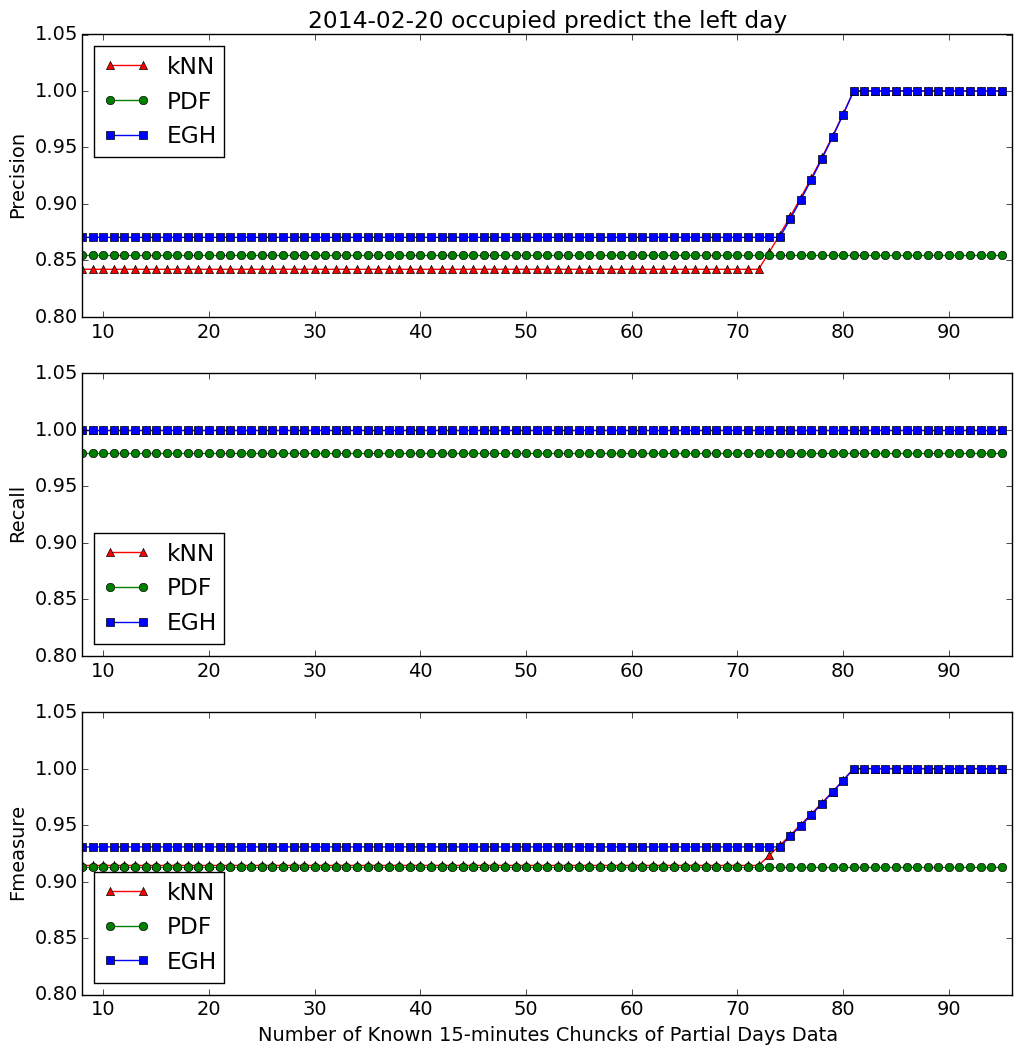
\includegraphics[width=1.0\textwidth]{adlfigs/study10person12014-02-20occupied.png}
\caption{Occupancy prediction precision, recall and f-measure comparison of three approaches 
of person1 on 02/20/2014 on Study10.}
\label{fig_study10}
\end{figure}
Figure~\ref{fig_study10} illustrates a person's occupancy prediction result on Study10.
There are three sub-figures. 
Each sub-figure describes the 
precision, recall, and f-measure 
of a person $person1$ on 02/20/2014. 
The blue line represents the mixture EGH model;
the green represents the PDF model;
the red denotes the kNN model. 
The x-axis is the number of known 15-minutes chunks of the test day. 
For instance, at $x=20$, 
we already know $20*15$ minutes' data 
and need to predict whether the in remaining $76$ chunks 
the home is occupied or not.
The y-axis denotes the precision, recall and f-measure values 
in the three sub-figures from top to down. 
The first sub-figure shows that  
the mixEGH has the highest precision, recall and F-measure on the test day 02/20/2014 
for occupancy prediction. The other two baseline approaches are comparable except that kNN performs better than PDF 
when the person comes back home after slot 72. 
Looking into the original data, we find that person1 actually comes later than usual 
in the training dataset. 
%In such case, mixture EGH performs best.  
%Figure \ref{fig_study10} (c) and (d) gives the occupancy and un-occupancy results 
%of person2 on 02/17/2014. 
%In such case, EGH mixture model performs best from the perspective of precision, recall and f-measure. 

\iffalse
Figure~\ref{fig_study14} (a) and (b) describe the case of person1 on 12/18/2013. 
Similar to Figure \ref{fig_study11} (a) and (b), 
mixture EGH model does not perform well before the person1 gets up 
and the reason keeps the same. 
The person1 slept late and some confused episodes are generated. 
Figure \ref{fig_study14} (c) and (d) describe the case of person1 on 12/19/2013. 
kNN performs better. Mixture EGH does not perform well because 12/19, 02/20 the person went out again after coming back and staying home for some time. However the training data don't include such case. 
\begin{figure}[h]
\centering
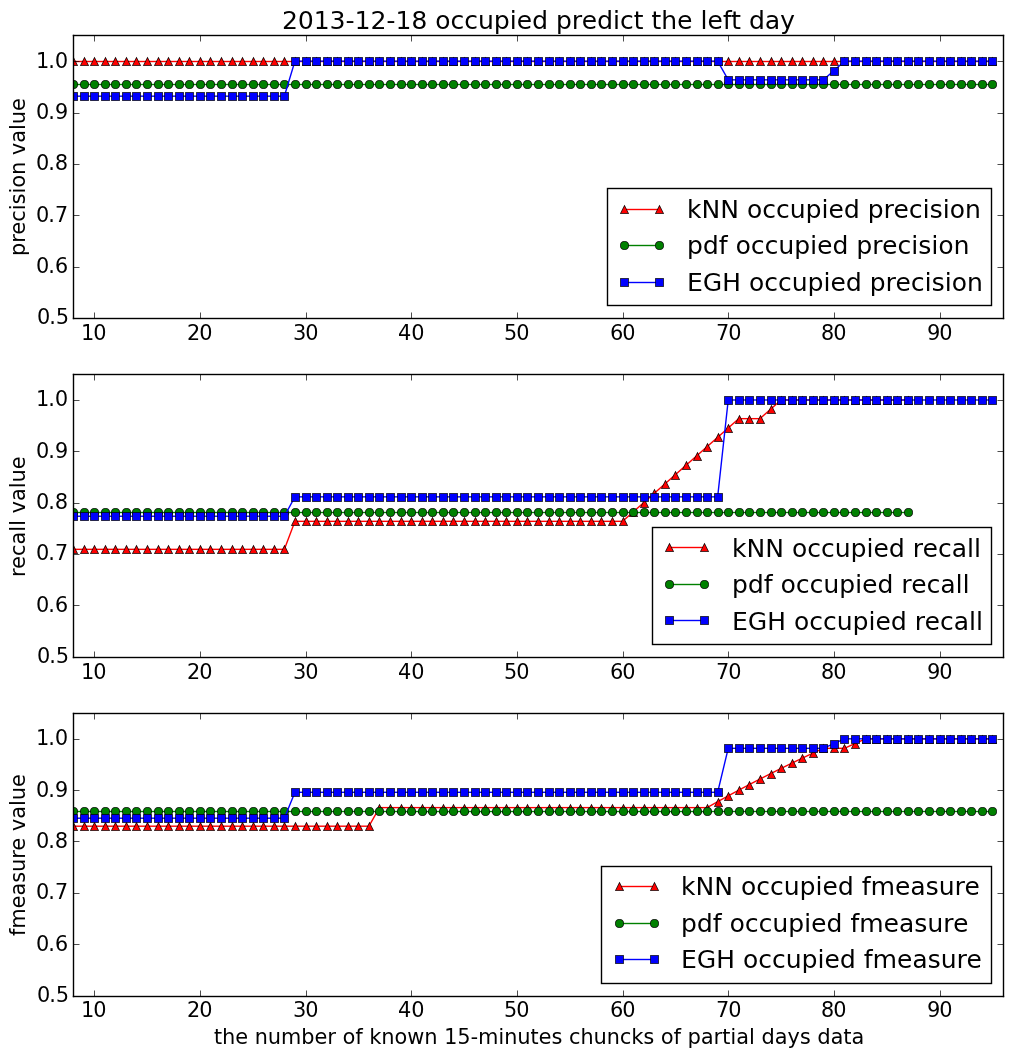
\includegraphics[width=0.5\textwidth]{adlfigs/study14person12013-12-18occupied.png} 
\caption{Study 14 Precision recall and f-measure comparison of three approaches.
person1 occupied 12/18/2014.}
\label{fig_study14}
\end{figure}
\fi


\subsection{Occupancy Prediction of Residential Buildings}
Based on individual prediction results, we deduce when a house is occupied
using logic OR operations on prediction results of two persons. 
The whole house occupancy prediction results are listed in 
table~\ref{tab_individualResults} and marked in bold. 
On Study10, the precision/recall/F-measure values of whole house are 0.92, 0.92 and 0.91, 
which are higher than the values from kNN approach 0.91, 0.90 and 0.91. Similarly mixture EGH model outperforms kNN in Study11. 
Note that in Study 11 on 02/04/2015, 
EGH does not perform as good as kNN on individuals
but performs a little bit better than kNN in occupancy prediction of the whole house. 
The reason behind that is because the actives of the two people inside home 
are not synchronized. The mixture EGH model can predict the 
occupancy for each person and grasp each person's activities more accurately. 
%When applying the logic OR operations on these two persons, 
%for whole-house occupancy prediction. 

\subsection{Limitations of Mixture EGH Model}
Although temporal mixture EGH model performs well on datasets Study10 and Study11, 
but not the same for the dataset Study14. 

\begin{table*}[!t]
%\vspace{0.2cm}
\hfill
%\begin{minipage}[t]{1.0\linewidth}%

\caption{Precision Recall F-measure of Individual and Whole House Occupancy Prediction in Study 14.}
\label{tab_resultsLimitation}
%\begin{center}
%\makebox[\textwidth]{
\centering
\small
\setlength\tabcolsep{2pt}
\begin{tabular} {|l|l|l|l|l|l|l|l|l|l|l|l|}
\hline
\multirow{2}{*}{Dataset}&\multirow{2}{*}{Date}&\multirow{2}{*}{Person} & \multicolumn{3}{|c|}{EGH}&\multicolumn{3}{|c|}{kNN} & \multicolumn{3}{|c|}{SVM} \\
\cline{4-12}
&&& precision & recall &fmeasure &precision & recall & fmeasure &precision & recall & fmeasure  \\
\hline
\multirow{3}{*}{study14}  & 12/18/2013 & person2&  \textbf{0.91} &  \textbf{0.91} &  \textbf{0.89} & 0.87 & 0.87 & 0.84 & 0.73 & 0.77 & 0.71\\
\cline{2-12}
& 12/18/2013 & person1&  \textbf{0.92} &  \textbf{0.92} &  \textbf{0.91} & 0.90 & 0.90 & 0.89 & 0.73 & 0.76 & 0.71 \\
\cline{2-12}
& 12/19/2014 & person2& 0.86 & 0.86 & 0.85  & \textbf{0.90} & \textbf{0.90} & \textbf{0.88} & 0.73 & 0.76 & 0.71\\
\cline{2-12}
& 12/19/2014 & person1& 0.85 & 0.84 & 0.84  & \textbf{0.86} & \textbf{0.86} & \textbf{0.85} & 0.73 & 0.76 & 0.71 \\
\cline{2-12}
& 12/20/2014 & person2& 0.92 & 0.94 & 0.92  & \textbf{0.98} & \textbf{0.97} & \textbf{0.97} & 0.75 & 0.79 & 0.75 \\
\cline{2-12}
& 12/20/2014 & person1& 0.90 & 0.91 & 0.90  & \textbf{0.95} & \textbf{0.95} & \textbf{0.95} & 0.75 & 0.79 & 0.75\\
\cline{2-12}
& 12/18/2013 & \textbf{wholehouse}&  \textbf{0.91}& \textbf{0.91} & \textbf{0.90} & 0.88	& 0.88 & 0.86 & 0.75 & 0.72 & 0.70 \\
\cline{2-12}
& 12/19/2013 & \textbf{wholehouse} & 0.841	& 0.845 & 0.838&  \textbf{0.848}& \textbf{0.853} & \textbf{0.842} & 0.79 & 0.74 & 0.74 \\
\cline{2-12}
& 12/20/2013 & \textbf{wholehouse} & 0.92	& 0.90 & 0.90&  \textbf{0.94}& \textbf{0.93} & \textbf{0.93} & 0.74 & 0.72 & 0.70 \\
\hline
\end{tabular}
%}
%\end{center}
%\end{minipage}%
%\hfill%
\end{table*}
Table~\ref{tab_resultsLimitation} shows that, 
in Study14, 
the mixture EGH model works better for the individual and whole-house occupancy prediction 
only on 12/18/2013 but not on 12/19/2013 and 12/20/2013. 
We check the activities of both individuals on these two days 
and find that both of them went out again 
after coming back and staying home for a while.
Since the episode of going out after coming back home from work 
do not occur frequently, mixture EGH cannot detect this pattern. Thus the occupancy prediction probability of these events 
is completely missing. However kNN performs better because it leverages all the 
historical data therefore, even if the abnormal event occurs once, 
this prediction approach incorporates it and obtains the average value. 

To relax the limitation of abnormal events, 
we propose a hybrid model for prediction:
when deploying this occupancy prediction in reality, 
for example for 30 minutes ahead prediction, 
just 15 minutes before prediction, if a person goes out again after coming back, 
the deployed system switches to the kNN approach other than mixture EGH model for prediction. In such case, this hybrid model can always get the best prediction results. 

\subsection{30 minutes Ahead House Occupancy Prediction with Hybrid Approach}
Preheating the house needs to evaluate how much time in advance to automatically turn on/off HVAC and the advance notice time estimation is given in~\cite{scott2011preheat}. 
Here we use 30 minutes ahead of time house occupancy prediction. 
%because it is reasonable for preheating. 
We compare the ROC curve of three approaches: mixture EGH model, kNN, and a hybrid approach of mixture EGH model and kNN. 
In this hybrid approach, 
we set mixture EGH results as the baseline, 
then replace the values of the mixture model by the values from kNN model 
in the following two situations: 
1) after a person comes back home; 2) the prediction probability of kNN is greater than 0.8. 
Figure~\ref{fig_rocresults_1}, ~\ref{fig_rocresults_2},~\ref{fig_rocresults_3}, illustrates the ROC curve of the whole house occupancy prediction on 02/20/2014 of dataset Study10, 02/04/2014 of dataset Study 11 
and 12/20/2013 of dataset Study14. 
The red and green represents the kNN and mixture EGH model, 
the blue denotes the hybrid approach. 
The ROC curves show that the hybrid approach always hold the largest area, namely 
0.96, 0.92 and 0.92, 
which indicate that the hybrid approach always performs the best. 
%\begin{figure*}[t]
	\centering{
		\begin{tabular}{cccc}		
		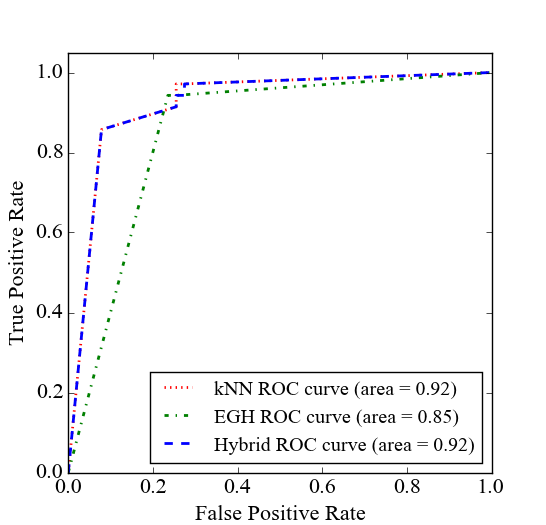
\includegraphics[width=0.33\textwidth]{adlfigs/study10ROC_02202014.png} &
		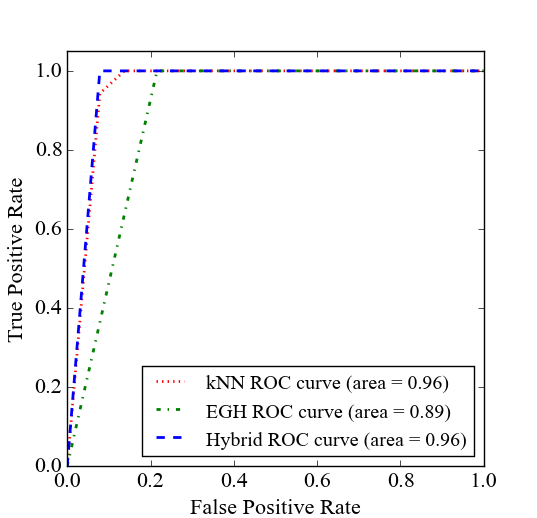
\includegraphics[width=0.33\textwidth]{adlfigs/study11ROC_02042014.png} &
		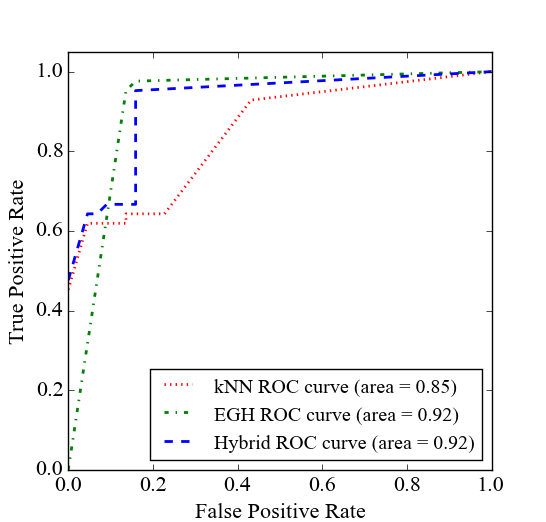
\includegraphics[width=0.33\textwidth]{adlfigs/study14ROC_12202013.png}
		\tabularnewline
		(a)&(b)&(c) \tabularnewline
		\end{tabular}
		}
	\caption{
	ROC curve of house occupancy prediction on 
(a) Study10 (02/20/2014). (b) Study11 (02/04/2014). (c) Study14 (12/20/2013).
}
	\label{fig_rocresults}
\end{figure*}
\begin{figure}[h]
	\centering{
		\begin{tabular}{cccc}		
		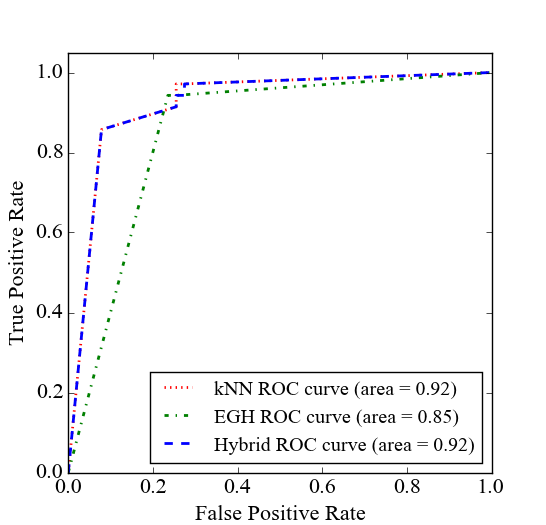
\includegraphics[width=0.7\textwidth]{adlfigs/study10ROC_02202014.png} &
		\tabularnewline
		(a)\tabularnewline
		\end{tabular}
		}
	\caption{
	ROC curve of house occupancy prediction on Study10 (02/20/2014).}
	\label{fig_rocresults_1}
\end{figure}

\begin{figure}[h]
	\centering{
		\begin{tabular}{cccc}		
		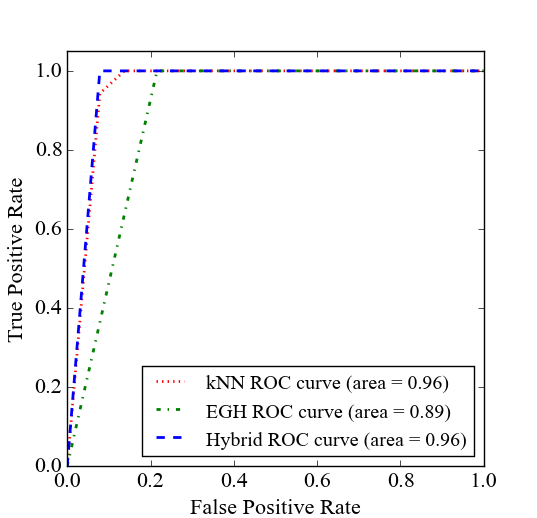
\includegraphics[width=0.7\textwidth]{adlfigs/study11ROC_02042014.png} &
		\tabularnewline
		((b)\tabularnewline
		\end{tabular}
		}
	\caption{
	ROC curve of house occupancy prediction on Study11 (02/04/2014).
}
	\label{fig_rocresults_2}
\end{figure}

\begin{figure}[h]
	\centering{
		\begin{tabular}{cccc}		
		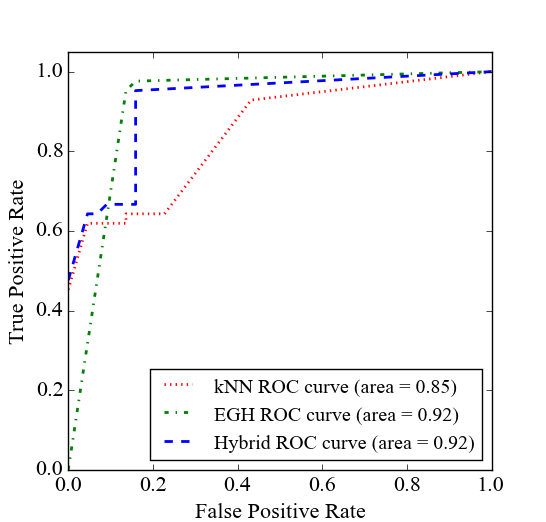
\includegraphics[width=0.7\textwidth]{adlfigs/study14ROC_12202013.png}
		\tabularnewline
		(c) \tabularnewline
		\end{tabular}
		}
	\caption{
	ROC curve of house occupancy prediction on (c) Study14 (12/20/2013).
}
	\label{fig_rocresults_3}
\end{figure}


%Also, we compare the 30 minutes whole house precision/recall/f-measure with the ROC curve, 
%the kNN ROC has a larger area even if EGH approach performs better on study10 and study11. 

%It depicts that ROC curve of mixture EGH model occupied larger area 0.92 than that from kNN approach 0.85. 
%We observe that although the precision/recall/fmeasure values are very close as in table~\ref{tab_individualResults}. 
%This hints that although the precision/recall/fmeasure results are competitive, 
%mixture EGH model can separate the occupancy and un-occupancy more sharply. 



%There are three test days in the dataset study14, 
%EGH outperforms kNN on the first day. 
%It's a tie on the second day. 
%The only exception on these datasets is the last day's experiment on study14, 
%kNN performs better because EGH mixture model currently
%only works on one-time even prediction. 



\chapter{Conclusion}

Smart buildings research involves many topics. 
We focus on two of them energy/water disaggregation and occupancy prediction. 
In this work, we utilize temporal mining algorithms 
frequent episode mining to discover the usage patterns 
of electrical devices and water use ends. 
Based on these frequent episodes, 
we can disaggregate individual devices from the multi-phases 
or single-phase aggregated data. 

Also, we mine the frequent episodes from the room position of a 
person in a residential building. 
Then we connect these frequent episodes with HMM 
to build Episode Generating HMM for target event unoccupancy prediction. 

In the future work, 
regarding energy disaggregation, we will incorporate more feature 
when a device starts up and improve this temporal mining 
approach to disaggregate more devices. 
For water disaggregation, since there's limitation in 
discovering specific water use ends, 
we will explore temporal mining approach, 
and integrate the dynamic time warping with motif mining. 

As to occupancy prediction, 
the hybrid approach by integrating kNN and a mixture of EGH 
performs best on sensor data set. 
Next step, we will apply this approach to GPS dataset 
on occupancy prediction. 


:
%
% The following two commands are all you need in the
% initial runs of your .tex file to
% produce the bibliography for the citations in your paper.
\bibliographystyle{abbrv}
\bibliography{reference}  % sigproc.bib is the name of the Bibliography in this case

% That's all folks!
\end{document}
